\section{Casi d'uso}
% TEMPLATE
%   \subsection{UC - NomeUseCase}
%   \label{sec:UC}
%   \includegraphics[]{diagramma_UML}
%   \begin{itemize}
	%       \item \textbf{Descrizione:} 
	%       \item \textbf{Attori:} 
	%       \item \textbf{Precondizioni:} 
	%       \item \textbf{Postcondizioni:} 
	%       \item \textbf{Scenario principale:} 
	%       \item \textbf{Generalizzazioni:} 
	%       \item \textbf{Estensioni:} 
	%   \end{itemize}

%   \hyperref[sec:UC]{\textbf{UC}}

% Link ad altre sezioni usando hyperref - utile per linkare generalizzazioni e estensioni
% La label fa da segnalibro a dove dovrà andare il link
%   \label{sec:nomeSezione}
% Link sul quale cliccare per andare alla label
%   \hyperref[sec:nomeSezione]{testo}
% END TEMPLATE

\subsection{Obiettivi}
La sezione ha come obiettivo quello di identificare e descrivere tutti i casi d'uso che sono stati individuati dal gruppo si sede di analisi del capitolato assegnato.

\subsection{Attori}
Il sistema dispone di due attori principali. In particolare:
\begin{itemize}
	\item \textbf{Utente}, che accede al servizio come utente in grado di selezionare una struttura database precaricata, inserire una frase di interrogazione in linguaggio naturale, visualizzare il prompt generato dall'LLM per poi confermarlo e ottenere una frase in formato SQL che rappresenti quello che era stato richiesto inizialmente.
	\item \textbf{Amministratore}, generalizzazione dell'utente generico ed accede al servizio come amministratore. Oltre a poter compiere tutte le azioni che può fare l'utente generico, l'amministratore può creare, visualizzare, modificare ed eliminare un database, le sue tabelle e i suoi campi.
\end{itemize}
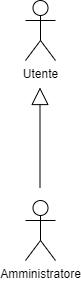
\includegraphics[scale=0.6]{UML_Use_Cases/UC-Attori.drawio.png}

\setcounter{secnumdepth}{0}

\subsection{UC1 - Login}
\label{sec:UC1}
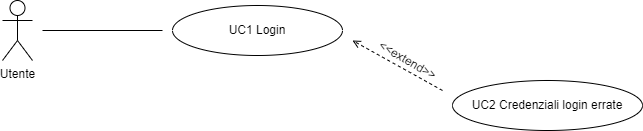
\includegraphics[scale=0.6]{UML_Use_Cases/UC1.drawio.png}
\begin{itemize}
	\item \textbf{Descrizione:} L’amministratore accede al pannello amministrativo con le sue credenziali;
	\item \textbf{Attori:} amministratore;
	\item \textbf{Precondizioni:} 
	\begin{itemize}
		\item L’amministratore possiede delle credenziali di accesso valide;
		\item L’amministratore non ha già effettuato l’accesso;
	\end{itemize}
	\item \textbf{Postcondizioni:} 
	\begin{itemize}
		\item L’utente Amministratore viene riconosciuto dal sistema;
	\end{itemize}
	\item \textbf{Scenario principale:} 
	\begin{itemize}
		\item L’ amministratore inserisce il proprio nome utente nel form di accesso (\hyperref[sec:UC1.1]{\textbf{UC1.1}});
		\item L’ amministratore inserisce la propria password nel form di accesso (\hyperref[sec:UC1.2]{\textbf{UC1.2}});
		\item Il sistema verifica che le credenziali ricevute siano corrette. 
	\end{itemize}
	\item \textbf{Estensioni:} Nel caso le credenziali non siano corrette:
	\begin{itemize}
		\item viene mostrato un errore - \hyperref[sec:UC2]{\textbf{UC2}}
	\end{itemize}
\end{itemize}

\subsubsection{UC1.1 - Inserimento nome utente}
\label{sec:UC1.1}
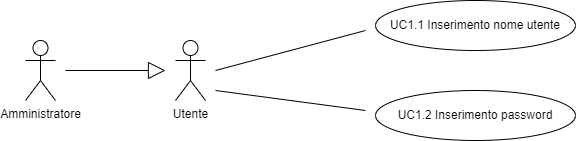
\includegraphics[scale=0.6]{UML_Use_Cases/UC1.1_1.2.drawio.png}
\begin{itemize}
	\item \textbf{Descrizione:} L’amministratore inserisce il proprio nome utente;
	\item \textbf{Attori:} amministratore;
	\item \textbf{Precondizioni:} 
	\begin{itemize}
		\item L’amministratore possiede le credenziali di accesso;
		\item L’amministratore non ha già effettuato l’accesso;
		\item L’amministratore sta effettuando il login (\hyperref[sec:UC1]{\textbf{UC1}})
	\end{itemize}
	\item \textbf{Postcondizioni:} 
	\begin{itemize}
		\item L’amministratore ha inserito correttamente il proprio nome utente;
	\end{itemize}
	\item \textbf{Scenario principale:} 
	\begin{itemize}
		\item L’amministratore inserisce il proprio nome utente nel form di accesso.
	\end{itemize}
\end{itemize}

\subsubsection{UC1.2 - Inserimento password}
\label{sec:UC1.2}
%\includegraphics[]{diagramma_UML}
\begin{itemize}
	\item \textbf{Descrizione:} L’amministratore inserisce la propria password;
	\item \textbf{Attori:} amministratore;
	\item \textbf{Precondizioni:} 
	\begin{itemize}
		\item L’amministratore possiede le credenziali di accesso;
		\item L’amministratore non ha già effettuato l’accesso;
		\item L’amministratore sta effettuando il login (\hyperref[sec:UC1]{\textbf{UC1}})
	\end{itemize}
	\item \textbf{Postcondizioni:} 
	\begin{itemize}
		\item L’amministratore ha inserito correttamente la propria password;
	\end{itemize}
	\item \textbf{Scenario principale:} 
	\begin{itemize}
		\item L’amministratore inserisce la propria password nel form di accesso.
	\end{itemize}
\end{itemize}

\subsection{UC2 - Credenziali login errate}
\label{sec:UC2}
%\includegraphics[]{diagramma_UML}
\begin{itemize}
	\item \textbf{Descrizione:} L’amministratore visualizza un messaggio di errore di autenticazione;
	\item \textbf{Attori:} amministratore;
	\item \textbf{Precondizioni:} 
	\begin{itemize}
		\item L’amministratore possiede le credenziali di accesso;
		\item L’amministratore non ha già effettuato l’accesso;
		\item L’amministratore sta effettuando il login (\hyperref[sec:UC1]{\textbf{UC1}});
		\item L’amministratore ha inserito il proprio nome utente (\hyperref[sec:UC1.1]{\textbf{UC1.1}});
		\item L’amministratore ha inserito la propria password (\hyperref[sec:UC1.2]{\textbf{UC1.2}});
	\end{itemize}
	\item \textbf{Postcondizioni:}
	\begin{itemize}
		\item L’amministratore non viene riconosciuto dal sistema e deve reinserire le proprie credenziali;
		\item L'amministrazione visualizza un messaggio di errore;
	\end{itemize}
	\item \textbf{Scenario principale:} 
	\begin{itemize}
		\item Il sistema verifica le credenziali ricevute siano corrette;
		\item Il sistema visualizza un messaggio di errore per le credenziali inserite se non corrette.
	\end{itemize}
\end{itemize}

\subsection{UC3 - Creazione Database}
\label{sec:UC3}
%\includegraphics[]{diagramma_UML}
\begin{itemize}
	\item \textbf{Descrizione:} l’amministratore vuole aggiungere la struttura di un database da poter interrogare;
	\item \textbf{Attori:} amministratore;
	\item \textbf{Precondizioni:} 
	\begin{itemize}
		\item L’amministratore ha effettuato il login (\hyperref[sec:UC1]{\textbf{UC1}});
		\item L’amministratore si trova nel pannello amministrativo;
	\end{itemize}
	\item \textbf{Postcondizioni:} 
	\begin{itemize}
		\item La struttura del database viene salvata nel programma;
	\end{itemize}
	\item \textbf{Scenario principale:} 
	\begin{itemize}
		\item L’amministratore inserisce il nome (\hyperref[sec:UC3.1]{\textbf{UC3.1}}) e la descrizione (\hyperref[sec:UC3.2]{\textbf{UC3.2}}) del database;
	\end{itemize}
	\item \textbf{Estensioni:} nel caso in cui venga inserito un nome già esistente:
	\begin{itemize}
		\item \hyperref[sec:UC4]{\textbf{UC4}} - Errore: nome Database già presente
	\end{itemize}
\end{itemize}

\subsubsection{UC3.1 - Inserimento nome Database}
\label{sec:UC3.1}
%\includegraphics[]{diagramma_UML}
\begin{itemize}
	\item \textbf{Descrizione:} l’amministratore deve inserire il nome del nuovo database da aggiungere;
	\item \textbf{Attori:} amministratore;
	\item \textbf{Precondizioni:} 
	\begin{itemize}
		\item L’amministratore ha effettuato il login (\hyperref[sec:UC1]{\textbf{UC1}});
		\item L’amministratore si trova nel pannello amministrativo;
		\item L’amministratore sta creando un nuovo database (\hyperref[sec:UC3]{\textbf{UC3}});
	\end{itemize}
	\item \textbf{Postcondizioni:} 
	\begin{itemize}
		\item L'amministratore ha inserito correttamente il nome del nuovo database;
	\end{itemize}
	\item \textbf{Scenario principale:} 
	\begin{itemize}
		\item L’amministratore inserisce il nome del database;
	\end{itemize}
\end{itemize}

\subsubsection{UC3.2 - Inserimento descrizione Database}
\label{sec:UC3.2}
%\includegraphics[]{diagramma_UML}
\begin{itemize}
	\item \textbf{Descrizione:} l’amministratore deve inserire la descrizione del nuovo database da aggiungere;
	\item \textbf{Attori:} amministratore;
	\item \textbf{Precondizioni:} 
	\begin{itemize}
		\item L’amministratore ha effettuato il login (\hyperref[sec:UC1]{\textbf{UC1}});
		\item L’amministratore si trova nel pannello amministrativo;
		\item L’amministratore sta creando un nuovo database (\hyperref[sec:UC3]{\textbf{UC3}});
	\end{itemize}
	\item \textbf{Postcondizioni:} 
	\begin{itemize}
		\item L'amministratore ha inserito correttamente la descrizione del nuovo database;
	\end{itemize}
	\item \textbf{Scenario principale:} 
	\begin{itemize}
		\item L’amministratore inserisce la descrizione del database;
	\end{itemize}
\end{itemize}

\subsection{UC4 - Errore: nome Database già presente}
\label{sec:UC4}
%\includegraphics[]{diagramma_UML}
\begin{itemize}
	\item \textbf{Descrizione:} L’amministratore visualizza un errore di creazione del database;
	\item \textbf{Attori:} amministratore;
	\item \textbf{Precondizioni:} 
	\begin{itemize}
		\item L’amministratore ha effettuato il login (\hyperref[sec:UC1]{\textbf{UC1}});
		\item L’amministratore si trova nel pannello amministrativo;
		\item L’amministratore sta creando un nuovo database (\hyperref[sec:UC3]{\textbf{UC3}});
	\end{itemize}
	\item \textbf{Postcondizioni:} 
	\begin{itemize}
		\item La struttura del database non viene salvata nel programma e l'amministratore visualizza un messaggio di errore;
	\end{itemize}
	\item \textbf{Scenario principale:} 
	\begin{itemize}
		\item L’amministratore inserisce il nome del database (\hyperref[sec:UC3.1]{\textbf{UC3.1}});
		\item L’amministratore inserisce la descrizione del database  (\hyperref[sec:UC3.2]{\textbf{UC3.2}});
		\item Il sistema verifica che non esista già un database con lo stesso nome;
		\item Il sistema visualizza un messaggio di errore per il nome inserito.
	\end{itemize}
\end{itemize}

\subsection{UC5 - Visualizzazione lista Strutture Database}
\label{sec:UC5}
%\includegraphics[]{diagramma_UML}
\begin{itemize}
	\item \textbf{Descrizione:} l’amministratore visualizza tutte le Strutture Database disponibili;
	\item \textbf{Attori:} amministratore;
	\item \textbf{Precondizioni:} 
	\begin{itemize}
		\item L’amministratore ha effettuato il login (\hyperref[sec:UC1]{\textbf{UC1}});
		\item L’amministratore si trova nel pannello amministrativo;
	\end{itemize}
	\item \textbf{Postcondizioni:} 
	\begin{itemize}
		\item L'amministratore può vedere nome e descrizione dei database presenti;
	\end{itemize}
	\item \textbf{Scenario principale:} 
	\begin{itemize}
		\item Il programma visualizza la lista dei database presenti, con la possibilità di modificarli, visualizzarli o eliminarli;
	\end{itemize}
\end{itemize}

\subsection{UC6 - Visualizzazione singola Struttura Database}
\label{sec:UC6}
%\includegraphics[]{diagramma_UML}
\begin{itemize}
	\item \textbf{Descrizione:} l’amministratore visualizza una Struttura Database;
	\item \textbf{Attori:} amministratore;
	\item \textbf{Precondizioni:} 
	\begin{itemize}
		\item L’amministratore ha effettuato il login (\hyperref[sec:UC1]{\textbf{UC1}});
		\item L’amministratore si trova nel pannello amministrativo;
		\item L'amministratore ha selezionato una Struttura Database dalla lista;
	\end{itemize}
	\item \textbf{Postcondizioni:} 
	\begin{itemize}
		\item L'amministratore visualizza il nome della Struttura Database;
		\item L'amministratore visualizza la descrizione della Struttura Database;
		\item L'amministratore visualizza la lista delle tabelle della Struttura Database  (\hyperref[sec:UC12]{\textbf{UC12}};
	\end{itemize}
	\item \textbf{Scenario principale:} 
	\begin{itemize}
		\item Il programma mostra la lista dei database presenti, con la possibilità di modificarli, visualizzarli o eliminarli;
	\end{itemize}
\end{itemize}


\subsection{UC7 - Modifica Struttura Database}
\label{sec:UC7}
%\includegraphics[]{diagramma_UML}
\begin{itemize}
	\item \textbf{Descrizione:} l’amministratore modifica la Strutture Database selezionata;
	\item \textbf{Attori:} amministratore;
	\item \textbf{Precondizioni:} 
	\begin{itemize}
		\item L’amministratore sta visualizzando una struttura Database (\hyperref[sec:UC6]{\textbf{UC6}});
	\end{itemize}
	\item \textbf{Postcondizioni:} 
	\begin{itemize}
		\item Il sistema aggiorna la Struttura Database;
	\end{itemize}
	\item \textbf{Scenario principale:} 
	\begin{itemize}
		\item Il sistema verifica il nome ricevuto;
		\item Il sistema ve
	\end{itemize}
\end{itemize}

\subsection{UC8 - Elimina Database}
\label{sec:UC8}
%\includegraphics[]{diagramma_UML}
\begin{itemize}
	\item \textbf{Descrizione:} l’amministratore elimina la Struttura Database selezionata;
	\item \textbf{Attori:} amministratore;
	\item \textbf{Precondizioni:} 
	\begin{itemize}
		\item L’amministratore ha effettuato il login (\hyperref[sec:UC1]{\textbf{UC1}});
		\item L’amministratore si trova nel pannello amministrativo;
		\item L’amministratore sta visualizzando la lista dei database (\hyperref[sec:UC5]{\textbf{UC5}});
	\end{itemize}
	\item \textbf{Postcondizioni:} 
	\begin{itemize}
		\item La Struttura Database selezionata viene eliminata dal sistema;
	\end{itemize}
	\item \textbf{Scenario principale:} 
	\begin{itemize}
		\item L'amministratore seleziona il database da eliminare usando il pulsante di eliminazione apposito;
		\item Il sistema visualizza un messaggio per chiedere la conferma dell'eliminazione;
		\item Se l'amministrazione conferma l'eliminazione, il database e le tabelle collegate verranno rimossi dal sistema e verrà visualizzato un messaggio di avvenuta eliminazione.
	\end{itemize}
\end{itemize}

\subsection{UC9 - Creazione tabella Database}
\label{sec:UC9}
%\includegraphics[]{diagramma_UML}
\begin{itemize}
	\item \textbf{Descrizione:} l’amministratore vuole aggiungere una tabella alla struttura del database da interrogare;
	\item \textbf{Attori:} amministratore;
	\item \textbf{Precondizioni:} 
	\begin{itemize}
		\item L’amministratore ha effettuato il login (\hyperref[sec:UC1]{\textbf{UC1}});
		\item L’amministratore si trova nel pannello amministrativo;
		\item L’amministratore si trova nella sezione di creazione di una nuova tabella;
	\end{itemize}
	\item \textbf{Postcondizioni:} 
	\begin{itemize}
		\item La tabella viene aggiunta alla struttura del database;
	\end{itemize}
	\item \textbf{Scenario principale:} 
	\begin{itemize}
		\item L’amministratore inserisce il nome, i sinonimi del nome e la descrizione della tabella;
	\end{itemize}
	\item \textbf{Generalizzazioni:} 
	\begin{itemize}
		\item \hyperref[sec:UC9.1]{\textbf{UC9.1}} - Inserimento nome tabella
		\item \hyperref[sec:UC9.2]{\textbf{UC9.2}} - Inserimento sinonimi tabella
		\item \hyperref[sec:UC9.3]{\textbf{UC9.3}} - Inserimento descrizione tabella
	\end{itemize}
	\item \textbf{Estensioni:} nel caso in cui non vengano inseriti i sinonimi del nome della tabella, o il nome esisti già:
	\begin{itemize}
		\item \hyperref[sec:UC9]{\textbf{UC9}} - Errore nella creazione della tabella
	\end{itemize}
\end{itemize}

\subsubsection{UC9.1 - Inserimento nome tabella}
\label{sec:UC9.1}
%\includegraphics[]{diagramma_UML}
\begin{itemize}
	\item \textbf{Descrizione:} l’amministratore inserisce il nome della tabella da creare;
	\item \textbf{Attori:} amministratore;
	\item \textbf{Precondizioni:} 
	\begin{itemize}
		\item L’amministratore ha effettuato il login (\hyperref[sec:UC1]{\textbf{UC1}});
		\item L’amministratore sta creando una nuova tabella (\hyperref[sec:UC9]{\textbf{UC9}});
	\end{itemize}
	\item \textbf{Postcondizioni:} 
	\begin{itemize}
		\item Il nome della tabella viene inserito nel form;
	\end{itemize}
	\item \textbf{Scenario principale:} 
	\begin{itemize}
		\item L’amministratore inserisce il nome della tabella nell'apposito form di creazione;
	\end{itemize}
\end{itemize}

\subsubsection{UC9.2 - Inserimento sinonimi tabella}
\label{sec:UC9.2}
%\includegraphics[]{diagramma_UML}
\begin{itemize}
	\item \textbf{Descrizione:} l’amministratore inserisce i sinonimi associati al nome della tabella da creare;
	\item \textbf{Attori:} amministratore;
	\item \textbf{Precondizioni:} 
	\begin{itemize}
		\item L’amministratore ha effettuato il login (\hyperref[sec:UC1]{\textbf{UC1}});
		\item L’amministratore sta creando una nuova tabella (\hyperref[sec:UC9]{\textbf{UC9}});
	\end{itemize}
	\item \textbf{Postcondizioni:} 
	\begin{itemize}
		\item I sinonimi del nome della tabella vengono inseriti nel form;
	\end{itemize}
	\item \textbf{Scenario principale:} 
	\begin{itemize}
		\item L’amministratore inserisce i sinonimi del nome della tabella nell'apposito form di creazione;
	\end{itemize}
\end{itemize}

\subsubsection{UC9.3 - Inserimento descrizione tabella}
\label{sec:UC9.3}
%\includegraphics[]{diagramma_UML}
\begin{itemize}
	\item \textbf{Descrizione:} l’amministratore inserisce la descrizione della tabella da creare;
	\item \textbf{Attori:} amministratore;
	\item \textbf{Precondizioni:} 
	\begin{itemize}
		\item L’amministratore ha effettuato il login (\hyperref[sec:UC1]{\textbf{UC1}});
		\item L’amministratore sta creando una nuova tabella (\hyperref[sec:UC9]{\textbf{UC9}});
	\end{itemize}
	\item \textbf{Postcondizioni:} 
	\begin{itemize}
		\item La descrizione della tabella viene inserita nel form;
	\end{itemize}
	\item \textbf{Scenario principale:} 
	\begin{itemize}
		\item L’amministratore inserisce la descrizione della tabella nell'apposito form di creazione;
	\end{itemize}
\end{itemize}

\subsection{UC10 - Errore nella creazione della tabella}
\label{sec:UC10}
%\includegraphics[]{diagramma_UML}
\begin{itemize}
	\item \textbf{Descrizione:} L’amministratore visualizza un errore di creazione della tabella;
	\item \textbf{Attori:} amministratore;
	\item \textbf{Precondizioni:} 
	\begin{itemize}
		\item L’amministratore ha effettuato il login (\hyperref[sec:UC1]{\textbf{UC1}});
		\item L’amministratore sta creando una nuova tabella (\hyperref[sec:UC9]{\textbf{UC9}});
	\end{itemize}
	\item \textbf{Postcondizioni:} 
	\begin{itemize}
		\item La tabella non viene creata e il programma visualizza un messaggio di errore;
	\end{itemize}
	\item \textbf{Scenario principale:} 
	\begin{itemize}
		\item L’amministratore inserisce il nome della tabella nel form di creazione (\hyperref[sec:UC8.1]{\textbf{UC8.1}});
		\item L’amministratore inserisce i sinonimi del nome della tabella nel form di creazione (\hyperref[sec:UC8.2]{\textbf{UC8.2}});
		\item L’amministratore inserisce la descrizione della tabella nel form di creazione (\hyperref[sec:UC8.3]{\textbf{UC8.3}});
		\item Il sistema verifica che non esista già una tabella con lo stesso nome e che vengano inseriti sinonimi e descrizione della tabella;
		\item Il sistema visualizza il messaggio di errore opportuno.
	\end{itemize}
\end{itemize}

\subsubsection{UC10.1 - Errore nome tabella già presente}
\label{sec:UC10.1}
%\includegraphics[]{diagramma_UML}
\begin{itemize}
	\item \textbf{Descrizione:} L’amministratore visualizza un errore relativo al nome della tabella;
	\item \textbf{Attori:} amministratore;
	\item \textbf{Precondizioni:} 
	\begin{itemize}
		\item L’amministratore ha effettuato il login (\hyperref[sec:UC1]{\textbf{UC1}});
		\item L’amministratore sta creando una nuova tabella (\hyperref[sec:UC9]{\textbf{UC9}});
	\end{itemize}
	\item \textbf{Postcondizioni:} 
	\begin{itemize}
		\item La tabella non viene creata e il programma visualizza un messaggio di errore;
	\end{itemize}
	\item \textbf{Scenario principale:} 
	\begin{itemize}
		\item Il sistema verifica che non esista già una tabella con lo stesso nome;
		\item Il sistema visualizza il messaggio di errore per il nome inserito.
	\end{itemize}
\end{itemize}

\subsubsection{UC10.2 - Errore sinonimi non inseriti}
\label{sec:UC10.2}
%\includegraphics[]{diagramma_UML}
\begin{itemize}
	\item \textbf{Descrizione:} L’amministratore visualizza un errore relativo ai sinonimi del nome della tabella;
	\item \textbf{Attori:} amministratore;
	\item \textbf{Precondizioni:} 
	\begin{itemize}
		\item L’amministratore ha effettuato il login (\hyperref[sec:UC1]{\textbf{UC1}});
		\item L’amministratore sta creando una nuova tabella (\hyperref[sec:UC9]{\textbf{UC9}});
	\end{itemize}
	\item \textbf{Postcondizioni:} 
	\begin{itemize}
		\item La tabella non viene creata e il programma visualizza un messaggio di errore;
	\end{itemize}
	\item \textbf{Scenario principale:} 
	\begin{itemize}
		\item Il sistema verifica che il campo relativo ai sinonimi del nome della tabella non sia vuoto;
		\item Il sistema visualizza il messaggio di errore per il campo sinonimi vuoto.
	\end{itemize}
\end{itemize}

\subsubsection{UC10.3 - Errore descrizione non inserita}
\label{sec:UC10.3}
%\includegraphics[]{diagramma_UML}
\begin{itemize}
	\item \textbf{Descrizione:} L’amministratore visualizza un errore relativo alla descrizione della tabella;
	\item \textbf{Attori:} amministratore;
	\item \textbf{Precondizioni:} 
	\begin{itemize}
		\item L’amministratore ha effettuato il login (\hyperref[sec:UC1]{\textbf{UC1}});
		\item L’amministratore sta creando una nuova tabella (\hyperref[sec:UC9]{\textbf{UC9}});
	\end{itemize}
	\item \textbf{Postcondizioni:} 
	\begin{itemize}
		\item La tabella non viene creata e il programma visualizza un messaggio di errore;
	\end{itemize}
	\item \textbf{Scenario principale:} 
	\begin{itemize}
		\item Il sistema verifica che il campo relativo ai sinonimi del nome della tabella non sia vuoto;
		\item Il sistema visualizza il messaggio di errore per il campo descrizione vuoto.
	\end{itemize}
\end{itemize}

\subsection{UC11 - Modifica della tabella}
\label{sec:UC11}
%\includegraphics[]{diagramma_UML}
\begin{itemize}
	\item \textbf{Descrizione:} l’amministratore vuole modificare una tabella del database selezionato e da interrogare;
	\item \textbf{Attori:} amministratore;
	\item \textbf{Precondizioni:} 
	\begin{itemize}
		\item L’amministratore ha effettuato il login (\hyperref[sec:UC1]{\textbf{UC1}});
		\item L’amministratore si trova nel pannello amministrativo;
		\item L’amministratore si trova nella sezione di modifica di una tabella;
	\end{itemize}
	\item \textbf{Postcondizioni:} 
	\begin{itemize}
		\item La tabella selezionata viene modificata;
	\end{itemize}
	\item \textbf{Scenario principale:} 
	\begin{itemize}
		\item L’amministratore modifica il nome, i sinonimi del nome e la descrizione della tabella;
	\end{itemize}
	\item \textbf{Estensioni:} nel caso in cui non vengano rimossi completamente i sinonimi del nome della tabella, o il nome modificato è già presente:
	\begin{itemize}
		\item \hyperref[sec:UC9]{\textbf{UC9}} - Errore nella creazione della tabella
	\end{itemize}
\end{itemize}

\subsection{UC12 - Visualizzazione lista delle tabella della Struttura Database}
\label{sec:UC12}
%\includegraphics[]{diagramma_UML}
\begin{itemize}
	\item \textbf{Descrizione:} l’amministratore visualizza tutte le tabelle della Struttura Database selezionata;
	\item \textbf{Attori:} amministratore;
	\item \textbf{Precondizioni:} 
	\begin{itemize}
		\item L’amministratore ha effettuato il login (\hyperref[sec:UC1]{\textbf{UC1}});
		\item L’amministratore si trova nel pannello amministrativo;
		\item L'amministratore ha selezionato una Struttura Database dalla lista;
	\end{itemize}
	\item \textbf{Postcondizioni:} 
	\begin{itemize}
		\item L'amministratore può vedere il nome delle tabelle presenti;
	\end{itemize}
	\item \textbf{Scenario principale:} 
	\begin{itemize}
		\item Il programma visualizza la lista delle tabelle presenti, con la possibilità di modificarle, visualizzarle o eliminarle;
	\end{itemize}
\end{itemize}

\subsection{UC13 - Visualizzazione della singola tabella}
\label{sec:UC13}
%\includegraphics[]{diagramma_UML}
\begin{itemize}
	\item \textbf{Descrizione:} l’amministratore visualizza la tabella della Struttura Database selezionata;
	\item \textbf{Attori:} amministratore;
	\item \textbf{Precondizioni:} 
	\begin{itemize}
		\item L'amministratore ha visualizzato la lista delle tabelle della Struttura Database (\hyperref[sec:UC12]{\textbf{UC12}});
		\item L'amministratore ha selezionato una tabella dalla lista;
	\end{itemize}
	\item \textbf{Postcondizioni:} 
	\begin{itemize}
		\item L'amministratore può vedere nome, descrizione e sinonimi della tabella selezionata;
		\item L'amministratore può visualizzare i campi della tabella selezionata;
	\end{itemize}
	\item \textbf{Scenario principale:} 
	\begin{itemize}
		\item Il programma visualizza i campi della tabella selezionata;
	\end{itemize}
\end{itemize}

\subsection{UC14 - Eliminazione della tabella}
\label{sec:UC14}
%\includegraphics[]{diagramma_UML}
\begin{itemize}
	\item \textbf{Descrizione:} l’amministratore elimina la tabella selezionata;
	\item \textbf{Attori:} amministratore;
	\item \textbf{Precondizioni:} 
	\begin{itemize}
		\item L’amministratore ha effettuato il login (\hyperref[sec:UC1]{\textbf{UC1}});
		\item L’amministratore si trova nel pannello amministrativo;
		\item L’amministratore sta visualizzando la lista delle tabelle (\hyperref[sec:UC12]{\textbf{UC12}});
	\end{itemize}
	\item \textbf{Postcondizioni:} 
	\begin{itemize}
		\item La Struttura Database selezionata viene eliminata dal sistema;
	\end{itemize}
	\item \textbf{Scenario principale:} 
	\begin{itemize}
		\item L'amministratore seleziona la tabella da eliminare usando il pulsante di eliminazione apposito;
		\item Il sistema visualizza un messaggio per chiedere la conferma dell'eliminazione;
		\item Se l'l'amministratore conferma l'eliminazione, la tabella e i suoi campi verranno rimossi dal sistema e verrà visualizzato un messaggio di avvenuta eliminazione.
	\end{itemize}
\end{itemize}

\subsection{UC15 - Creazione campo tabella}
\label{sec:UC15}
%\includegraphics[]{diagramma_UML}
\begin{itemize}
	\item \textbf{Descrizione:} l’amministratore vuole aggiungere un campo alla tabella selezionata;
	\item \textbf{Attori:} amministratore;
	\item \textbf{Precondizioni:} 
	\begin{itemize}
		\item L’amministratore ha effettuato il login (\hyperref[sec:UC1]{\textbf{UC1}});
		\item L’amministratore si trova nel pannello amministrativo;
		\item L’amministratore si trova nella sezione di visualizzazione di una tabella (\hyperref[sec:UC13]{\textbf{UC13}});
		\item L’amministratore sta inserendo i campi che compongono la tabella;
	\end{itemize}
	\item \textbf{Postcondizioni:} 
	\begin{itemize}
		\item I campi vengono aggiunti alla tabella;
	\end{itemize}
	\item \textbf{Scenario principale:} 
	\begin{itemize}
		\item L’amministratore inserisce il nome del campo \hyperref[sec:UC15.1]{\textbf{UC15.1}};
		\item L'amministratore seleziona il tipo del campo \hyperref[sec:UC15.2]{\textbf{UC15.2}};
		\item L'amministratore inserisce i sinonimi del campo \hyperref[sec:UC15.3]{\textbf{UC15.3}};
	\end{itemize}
	\item \textbf{Estensioni:} nel caso in cui il nome inserito sia già esistente o non sia stato selezionato il tipo o inseriti i sinonimi:
	\begin{itemize}
		\item \hyperref[sec:UC16]{\textbf{UC16}} - Errore creazione campo
	\end{itemize}
\end{itemize}

\subsubsection{UC15.1 - Inserimento nome campo}
\label{sec:UC15.1}
%\includegraphics[]{diagramma_UML}
\begin{itemize}
	\item \textbf{Descrizione:} l’amministratore vuole inserire il nome del campo da inserire nella tabella;
	\item \textbf{Attori:} amministratore;
	\item \textbf{Precondizioni:} 
	\begin{itemize}
		\item L’amministratore ha effettuato il login (\hyperref[sec:UC1]{\textbf{UC1}});
		\item L’amministratore si trova nel pannello amministrativo;
		\item L’amministratore si trova nella sezione di visualizzazione di una tabella (\hyperref[sec:UC13]{\textbf{UC13}});
		\item L’amministratore sta inserendo i campi che compongono la tabella;
	\end{itemize}
	\item \textbf{Postcondizioni:} 
	\begin{itemize}
		\item Il nome del campo viene inserito;
	\end{itemize}
	\item \textbf{Scenario principale:} 
	\begin{itemize}
		\item L’amministratore inserisce il nome del campo nella casella di testo dedicata;
	\end{itemize}
	\item \textbf{Estensioni:} nel caso in cui il nome inserito sia già esistente:
	\begin{itemize}
		\item \hyperref[sec:UC16.1]{\textbf{UC16.1}} - Errore nome campo già esistente
	\end{itemize}
\end{itemize}

\subsubsection{UC15.2 - Inserimento tipo campo}
\label{sec:UC15.2}
%\includegraphics[]{diagramma_UML}
\begin{itemize}
	\item \textbf{Descrizione:} l’amministratore vuole selezionare il tipo del campo da inserire nella tabella;
	\item \textbf{Attori:} amministratore;
	\item \textbf{Precondizioni:} 
	\begin{itemize}
		\item L’amministratore ha effettuato il login (\hyperref[sec:UC1]{\textbf{UC1}});
		\item L’amministratore si trova nel pannello amministrativo;
		\item L’amministratore si trova nella sezione di visualizzazione di una tabella (\hyperref[sec:UC13]{\textbf{UC13}}) ;
		\item L’amministratore sta inserendo i campi che compongono la tabella;
	\end{itemize}
	\item \textbf{Postcondizioni:} 
	\begin{itemize}
		\item Il tipo del campo viene selezionato;
	\end{itemize}
	\item \textbf{Scenario principale:} 
	\begin{itemize}
		\item L’amministratore sceglie il tipo di campo, selezionandolo dalle scelte possibili;
	\end{itemize}
	\item \textbf{Estensioni:} nel caso in cui il tipo non venga selezionato:
	\begin{itemize}
		\item \hyperref[sec:UC16.2]{\textbf{UC16.2}} - Errore tipo campo non selezionato
	\end{itemize}
\end{itemize}

\subsubsection{UC15.3 - Inserimento sinonimi campo}
\label{sec:UC15.3}
%\includegraphics[]{diagramma_UML}
\begin{itemize}
	\item \textbf{Descrizione:} l’amministratore vuole inserire i sinonimi del campo da inserire nella tabella;
	\item \textbf{Attori:} amministratore;
	\item \textbf{Precondizioni:} 
	\begin{itemize}
		\item L’amministratore ha effettuato il login (\hyperref[sec:UC1]{\textbf{UC1}});
		\item L’amministratore si trova nel pannello amministrativo;
		\item L’amministratore si trova nella sezione di visualizzazione di una tabella (\hyperref[sec:UC13]{\textbf{UC13}} ;
		\item L’amministratore sta inserendo i campi che compongono la tabella;
	\end{itemize}
	\item \textbf{Postcondizioni:} 
	\begin{itemize}
		\item I sinonimi del nome del campo vengono inseriti;
	\end{itemize}
	\item \textbf{Scenario principale:} 
	\begin{itemize}
		\item L’amministratore inserisce i sinonimi del nome del campo nella casella di testo dedicata;
	\end{itemize}
	\item \textbf{Estensioni:} nel caso in cui i sinonimi non vengano inseriti:
	\begin{itemize}
		\item \hyperref[sec:UC16.3]{\textbf{UC16.3}} - Errore mancato inserimento sinonimi campo
	\end{itemize}
\end{itemize}

\subsection{UC16 - Errore creazione campo}
\label{sec:UC16}
%\includegraphics[]{diagramma_UML}
\begin{itemize}
	\item \textbf{Descrizione:} L’amministratore visualizza un errore di creazione del campo;
	\item \textbf{Attori:} amministratore;
	\item \textbf{Precondizioni:} 
	\begin{itemize}
		\item L’amministratore ha effettuato il login (\hyperref[sec:UC1]{\textbf{UC1}});
		\item L’amministratore si trova nel pannello amministrativo;
		\item L’amministratore si trova nella sezione di visualizzazione di una tabella (\hyperref[sec:UC13]{\textbf{UC13}} ;
		\item L’amministratore sta creando un nuovo campo (\hyperref[sec:UC15]{\textbf{UC15}});
	\end{itemize}
	\item \textbf{Postcondizioni:} 
	\begin{itemize}
		\item Il campo non viene creato e il programma visualizza un messaggio di errore;
	\end{itemize}
	\item \textbf{Scenario principale:} 
	\begin{itemize}
		\item L’amministratore inserisce il nome del campo nel form di creazione (\hyperref[sec:UC15.1]{\textbf{UC15.1}});
		\item L’amministratore seleziona il tipo del campo nel form di creazione (\hyperref[sec:UC15.2]{\textbf{UC15.2}});
		\item L’amministratore inserisce i sinonimi del nome campo nel form di creazione (\hyperref[sec:UC15.3]{\textbf{UC15.3}});
		\item Il sistema verifica che non esista già una tabella con lo stesso nome, che venga selezionato il tipo e che vengano inseriti i sinonimi del campo;
		\item Il sistema visualizza il messaggio di errore opportuno.
	\end{itemize}
\end{itemize}

\subsubsection{UC16.1 - Errore nome campo già esistente}
\label{sec:UC16.1}
%\includegraphics[]{diagramma_UML}
\begin{itemize}
	\item \textbf{Descrizione:} L’amministratore visualizza un errore relativo al nome del campo;
	\item \textbf{Attori:} amministratore;
	\item \textbf{Precondizioni:} 
	\begin{itemize}
		\item L’amministratore ha effettuato il login (\hyperref[sec:UC1]{\textbf{UC1}});
		\item L’amministratore si trova nel pannello amministrativo;
		\item L’amministratore si trova nella sezione di visualizzazione di una tabella (\hyperref[sec:UC13]{\textbf{UC13}} ;
		\item L’amministratore sta creando un nuovo campo (\hyperref[sec:UC15]{\textbf{UC15}});
	\end{itemize}
	\item \textbf{Postcondizioni:} 
	\begin{itemize}
		\item Il campo non viene creato e il programma visualizza un messaggio di errore;
	\end{itemize}
	\item \textbf{Scenario principale:} 
	\begin{itemize}
		\item Il sistema verifica che non esista già un campo con lo stesso nome;
		\item Il sistema visualizza il messaggio di errore per il nome inserito.
	\end{itemize}
\end{itemize}

\subsubsection{UC16.2 - Errore tipo campo non selezionato}
\label{sec:UC16.2}
%\includegraphics[]{diagramma_UML}
\begin{itemize}
	\item \textbf{Descrizione:} L’amministratore visualizza un errore relativo al tipo del campo;
	\item \textbf{Attori:} amministratore;
	\item \textbf{Precondizioni:} 
	\begin{itemize}
		\item L’amministratore ha effettuato il login (\hyperref[sec:UC1]{\textbf{UC1}});
		\item L’amministratore si trova nel pannello amministrativo;
		\item L’amministratore si trova nella sezione di visualizzazione di una tabella (\hyperref[sec:UC13]{\textbf{UC13}} ;
		\item L’amministratore sta creando un nuovo campo (\hyperref[sec:UC15]{\textbf{UC15}});
	\end{itemize}
	\item \textbf{Postcondizioni:} 
	\begin{itemize}
		\item Il campo non viene creato e il programma visualizza un messaggio di errore;
	\end{itemize}
	\item \textbf{Scenario principale:} 
	\begin{itemize}
		\item Il sistema verifica che sia stato selezionato un tipo tra quelli disponibili per il campo;
		\item Il sistema visualizza il messaggio di errore per il tipo del campo.
	\end{itemize}
\end{itemize}

\subsubsection{UC16.3 - Errore mancato inserimento sinonimi campo}
\label{sec:UC16.3}
%\includegraphics[]{diagramma_UML}
\begin{itemize}
	\item \textbf{Descrizione:} L’amministratore visualizza un errore relativo ai sinonimi del nome del campo;
	\item \textbf{Attori:} amministratore;
	\item \textbf{Precondizioni:} 
	\begin{itemize}
		\item L’amministratore ha effettuato il login (\hyperref[sec:UC1]{\textbf{UC1}});
		\item L’amministratore si trova nel pannello amministrativo;
		\item L’amministratore si trova nella sezione di visualizzazione di una tabella (\hyperref[sec:UC13]{\textbf{UC13}} ;
		\item L’amministratore sta creando un nuovo campo (\hyperref[sec:UC15]{\textbf{UC15}});
	\end{itemize}
	\item \textbf{Postcondizioni:} 
	\begin{itemize}
		\item Il campo non viene creato e il programma visualizza un messaggio di errore;
	\end{itemize}
	\item \textbf{Scenario principale:} 
	\begin{itemize}
		\item Il sistema verifica che siano stati inseriti dei sinonimi per il nome del campo;
		\item Il sistema visualizza il messaggio di errore per i sinonimi.
	\end{itemize}
\end{itemize}

\subsection{UC17 - Visualizzazione lista dei campi della tabella}
\label{sec:UC17}
%\includegraphics[]{diagramma_UML}
\begin{itemize}
	\item \textbf{Descrizione:} l’amministratore visualizza tutti i campi della tabella selezionata;
	\item \textbf{Attori:} amministratore;
	\item \textbf{Precondizioni:} 
	\begin{itemize}
		\item L’amministratore ha effettuato il login (\hyperref[sec:UC1]{\textbf{UC1}});
		\item L’amministratore si trova nella sezione di visualizzazione di una tabella (\hyperref[sec:UC13]{\textbf{UC13}} ;
		\item L’amministratore si trova nel pannello amministrativo;
	\end{itemize}
	\item \textbf{Postcondizioni:} 
	\begin{itemize}
		\item L'amministratore può vedere nome, tipo e sinonimi dei campi presenti;
	\end{itemize}
	\item \textbf{Scenario principale:} 
	\begin{itemize}
		\item Il programma visualizza la lista dei campi presenti, con la possibilità di modificarli, visualizzarli o eliminarli;
	\end{itemize}
\end{itemize}

\subsection{UC18 - Visualizzazione singolo campo tabella}
\label{sec:UC18}
%\includegraphics[]{diagramma_UML}
\begin{itemize}
	\item \textbf{Descrizione:} l’amministratore visualizza tutti i campi della tabella selezionata;
	\item \textbf{Attori:} amministratore;
	\item \textbf{Precondizioni:} 
	\begin{itemize}
		\item L’amministratore ha effettuato il login (\hyperref[sec:UC1]{\textbf{UC1}});
		\item L’amministratore si trova nella sezione di visualizzazione di una tabella (\hyperref[sec:UC13]{\textbf{UC13}});
		\item L’amministratore si trova nel pannello amministrativo;
		\item L'amministratore ha selezionato un campo di una tabella;
	\end{itemize}
	\item \textbf{Postcondizioni:} 
	\begin{itemize}
		\item L'amministratore può vedere nome, tipo e sinonimi del campo selezionatoi;
	\end{itemize}
	\item \textbf{Scenario principale:} 
	\begin{itemize}
		\item Il programma visualizza la lista dei campi presenti, con la possibilità di modificarli, visualizzarli o eliminarli;
	\end{itemize}
\end{itemize}

\subsection{UC19 - Modifica campo tabella}
\label{sec:UC19}
%\includegraphics[]{diagramma_UML}
\begin{itemize}
	\item \textbf{Descrizione:} l’amministratore vuole modificare un campo alla tabella selezionata;
	\item \textbf{Attori:} amministratore;
	\item \textbf{Precondizioni:} 
	\begin{itemize}
		\item L’amministratore ha effettuato il login (\hyperref[sec:UC1]{\textbf{UC1}});
		\item L’amministratore si trova nel pannello amministrativo;
		\item L’amministratore si trova nella sezione di visualizzazione di una tabella (\hyperref[sec:UC13]{\textbf{UC13}});
		\item L’amministratore sta modificando i campi che compongono la tabella;
	\end{itemize}
	\item \textbf{Postcondizioni:} 
	\begin{itemize}
		\item I campi della tabella vengono modificati;
	\end{itemize}
	\item \textbf{Scenario principale:} 
	\begin{itemize}
		\item L’amministratore inserisce il nome del campo \hyperref[sec:UC15.1]{\textbf{UC15.1}};
		\item L'amministratore seleziona il tipo del campo \hyperref[sec:UC15.2]{\textbf{UC15.2}};
		\item L'amministratore inserisce i sinonimi del campo \hyperref[sec:UC15.3]{\textbf{UC15.3}};
	\end{itemize}

		\item \textbf{Estensioni:} nel caso in cui il nome inserito sia già esistente o non sia stato selezionato il tipo o inseriti i sinonimi:
		\begin{itemize}
			\item (\hyperref[sec:UC16]{\textbf{UC16}}) - Errore creazione campo
	\end{itemize}
\end{itemize}


\subsection{UC20 - Eliminazione campo tabella}
\label{sec:UC20}
%\includegraphics[]{diagramma_UML}
\begin{itemize}
	\item \textbf{Descrizione:} l’amministratore elimina il campo selezionato;
	\item \textbf{Attori:} amministratore;
	\item \textbf{Precondizioni:} 
	\begin{itemize}
		\item L’amministratore ha effettuato il login (\hyperref[sec:UC1]{\textbf{UC1}});
		\item L’amministratore si trova nel pannello amministrativo;
		\item L’amministratore sta visualizzando la lista dei campi (\hyperref[sec:UC15]{\textbf{UC15}});
	\end{itemize}
	\item \textbf{Postcondizioni:} 
	\begin{itemize}
		\item Il campo selezionato viene eliminato dal sistema;
	\end{itemize}
	\item \textbf{Scenario principale:} 
	\begin{itemize}
		\item L'amministratore seleziona il campo da eliminare;
		\item Il sistema visualizza un messaggio per chiedere la conferma dell'eliminazione;
		\item Se l'amministrazione conferma l'eliminazione, il campo verrà rimosso dal sistema e verrà visualizzato un messaggio di avvenuta eliminazione.
	\end{itemize}
\end{itemize}

\subsection{UC21 - Caricamento struttura Database tramite file}
\label{sec:UC21}
\begin{itemize}
	\item \textbf{Descrizione:} l’amministratore vuole caricare un file che descrive una Struttura Database;
	\item \textbf{Attori:} amministratore;
	\item \textbf{Precondizioni:} 
	\begin{itemize}
		\item L’amministratore ha effettuato il login (\hyperref[sec:UC1]{\textbf{UC1}});
		\item L’amministratore si trova nel pannello amministrativo;
	\end{itemize}
	\item \textbf{Postcondizioni:} 
	\begin{itemize}
		\item La Struttura Database viene caricata correttamente nel sistema;
	\end{itemize}
	\item \textbf{Scenario principale:} 
	\begin{itemize}
		\item L'amministrazione inserisce il file della Struttura Database;
	\end{itemize}
	\item \textbf{Estensioni:} nel caso il file non sia corretto:
	\begin{itemize}
		\item \hyperref[sec:UC22]{\textbf{UC22}} - Errore caricamento file
	\end{itemize}
\end{itemize}

\subsection{UC22 - Errore caricamento file}
\label{sec:UC22}
\begin{itemize}
	\item \textbf{Descrizione:} L’amministratore visualizza un errore di caricamento del file;
	\item \textbf{Attori:} amministratore;
	\item \textbf{Precondizioni:} 
	\begin{itemize}
		\item L’amministratore ha effettuato il login (\hyperref[sec:UC1]{\textbf{UC1}});
		\item L’amministratore si trova nel pannello amministrativo;
		\item L’amministratore sta caricando un file Struttura del Databese (\hyperref[sec:UC21]{\textbf{UC21}});
	\end{itemize}
	\item \textbf{Postcondizioni:} 
	\begin{itemize}
		\item La tabella non viene creata e il programma visualizza un messaggio di errore;
	\end{itemize}
	\item \textbf{Scenario principale:} 
	\begin{itemize}
		\item Il sistema verifica che il formato del file sia corretto;
		\item Il sistema mostra un messaggio di errore se il formato non è corretto;
	\end{itemize}
\end{itemize}


\subsection{UC23 - Logout}
\label{sec:UC23}
%\includegraphics[]{diagramma_UML}
\begin{itemize}
	\item \textbf{Descrizione: l'amministratore vuole fare il logout dall'area amministrativa} 
	\item \textbf{Attori:} amministratore;
	\item \textbf{Precondizioni:} 
	\begin{itemize}
		\item L’amministratore ha effettuato il login (\hyperref[sec:UC1]{\textbf{UC1}});
	\end{itemize}
	\item \textbf{Postcondizioni:} 
	\begin{itemize}
		\item Viene visualizzata la pagina iniziale;
	\end{itemize}
	\item \textbf{Scenario principale:} 
	\begin{itemize}
		\item L’amministratore clicca il pulsante di logout;
		\item L’amministratore viene reindirizzato alla pagina iniziale.
	\end{itemize}
	\item \textbf{Estensioni:} nel caso in cui l'utente non fosse loggato:
	\begin{itemize}
		\item Viene visualizzato un errore - \hyperref[sec:UC24]{\textbf{UC24}}.
	\end{itemize}
\end{itemize}

\subsection{UC24 - Errore logout}
\label{sec:UC24}

\subsection{UC25 - Selezione Struttura Database da interrogare}
\label{sec:UC25}
%\includegraphics[]{diagramma_UML}
\begin{itemize}
	\item \textbf{Descrizione:} l’utente seleziona la Struttura Database che vuole interrogare da una lista;
	\item \textbf{Attori:} utente;
	\item \textbf{Precondizioni:}
	\begin{itemize}
		\item Sono presenti una o più Strutture Database da poter selezionare;
	\end{itemize}
	\item \textbf{Postcondizioni:}
	\begin{itemize}
		\item L’utente ha selezionato una Struttura Database;
	\end{itemize}
	\item \textbf{Scenario principale:}
	\begin{itemize}
		\item L’utente ha il programma aperto;
		\item L’utente seleziona uno dei database presenti nella lista.
	\end{itemize}
	\item \textbf{Estensioni:} In caso l'utente non selezioni una Strttura Database;
	\begin{itemize}
		\item Errore Struttura Database non selezionata (\hyperref[sec:UC26]{\textbf{UC26}});
	\end{itemize}
\end{itemize}

\subsection{UC26 - Errore Struttura Database non selezionata}
\label{sec:UC26}
\begin{itemize}
	\item \textbf{Descrizione:} l’utente non ha selezionato una Struttura Database;
	\item \textbf{Attori:} utente;
	\item \textbf{Precondizioni:}
	\begin{itemize}
		\item Sono presenti una o più Strutture Database da poter selezionare;
	\end{itemize}
	\item \textbf{Postcondizioni:}
	\begin{itemize}
		\item L’utente visualizza un messaggio di errore;
	\end{itemize}
	\item \textbf{Scenario principale:}
	\begin{itemize}
		\item Il sistema non riceve una Struttura Database;
		\item Il sistema mostra un errore;
	\end{itemize}
\end{itemize}

\subsection{UC27 - Inserimento frase in linguaggio naturale}
\label{sec:UC27}
%\includegraphics[]{diagramma_UML}
\begin{itemize}
	\item \textbf{Descrizione:} L’utente scrive una frase in linguaggio naturale;
	\item \textbf{Attori:} utente;
	\item \textbf{Precondizioni:} 
	\begin{itemize}
		\item L’utente ha selezionato un file di struttura Database (\hyperref[sec:UC25]{\textbf{UC25}});
	\end{itemize}
	\item \textbf{Postcondizioni:} 
	\begin{itemize}
		\item L’utente riceve un prompt per la creazione della query richiesta (\hyperref[sec:UC29]{\textbf{UC29}});
	\end{itemize}
	\item \textbf{Scenario principale:} 
	\begin{itemize}
		\item L’utente ha il programma aperto;
		\item L’utente seleziona la casella di testo;
		\item L’utente scrive la frase per interrogare il database;
		\item L’utente clicca il pulsante apposito per ottenere il prompt.
	\end{itemize}
	\item \textbf{Estensioni:} nel caso in cui venga inserita una frase non inerente al database, o non comprensibile:
	\begin{itemize}
		\item Viene visualizzato un errore - \hyperref[sec:UC28]{\textbf{UC28}}.
	\end{itemize}
\end{itemize}

\subsection{UC28 - Errore frase naturale}
\label{sec:UC28}
\begin{itemize}
	\item \textbf{Descrizione:} L’utente visualizza un errore inerente alla frase inserita;
	\item \textbf{Attori:} utente;
	\item \textbf{Precondizioni:} 
	\begin{itemize}
		\item L’utente ha selezionato un file di struttura Database (\hyperref[sec:UC25]{\textbf{UC25}});
		\item L'utente ha inserito una frase in linguaggio naturale (\hyperref[sec:UC27]{\textbf{UC27}});
	\end{itemize}
	\item \textbf{Postcondizioni:} 
	\begin{itemize}
		\item L’utente visualizza un messaggio di errore;
	\end{itemize}
	\item \textbf{Scenario principale:} 
	\begin{itemize}
		\item Il sistema verifica la frase ricevuta;
		\item Il sistema non riescie ad elaborare la frase;
		\item Il sistema visualizza un messaggio di errore.
	\end{itemize}
	\end{itemize}


\subsubsection{UC28.1 - Errore frase non inserita}
\label{sec:UC28.1}
\begin{itemize}
	\item \textbf{Descrizione:} L’utente visualizza un errore relativo alla frase inserita;
	\item \textbf{Attori:} utente;
	\item \textbf{Precondizioni:} 
	\begin{itemize}
		\item L’utente ha selezionato un file di struttura Database (\hyperref[sec:UC25]{\textbf{UC25}});
		\item L'utente ha inserito una frase in linguaggio naturale (\hyperref[sec:UC27]{\textbf{UC27}});
	\end{itemize}
	\item \textbf{Postcondizioni:} 
	\begin{itemize}
		\item Il programma mostra un messaggio di errore;
		\item Il prompt non viene generato;
	\end{itemize}
	\item \textbf{Scenario principale:} 
	\begin{itemize}
		\item Il sistema non ha ricevuto una frase;
		\item Il sistema visualizza un messaggio di errore.
	\end{itemize}
\end{itemize}


\subsubsection{UC28.2 - Errore frase non compresa}
\label{sec:UC28.2}
\begin{itemize}
	\item \textbf{Descrizione:} L’utente inserisce una frase in linguaggio naturale non comprensibile dal sistema;
	\item \textbf{Attori:} utente;
	\item \textbf{Precondizioni:} 
	\begin{itemize}
		\item L’utente ha selezionato un file di struttura Database (\hyperref[sec:UC25]{\textbf{UC25}});
		\item L'utente ha inserito una frase in linguaggio naturale (\hyperref[sec:UC27]{\textbf{UC27}});
	\end{itemize}
	\item \textbf{Postcondizioni:} 
	\begin{itemize}
		\item Il programma mostra un messaggio di errore;
		\item Il prompt non viene generato;
	\end{itemize}
	\item \textbf{Scenario principale:} 
	\begin{itemize}
		\item Il sistema verifica la frase ricevuta;
		\item Il sistema non comprende la frase;
		\item Il sistema visualizza un messaggio di errore.
	\end{itemize}
\end{itemize}


\subsubsection{UC28.3 - Errore frase non inerente}
\label{sec:UC28.3}
%\includegraphics[]{diagramma_UML}
\begin{itemize}
	\item \textbf{Descrizione:} l’utente inserisce una frase in linguaggio naturale non interpretabile dal sistema come inerente al database;
	\item \textbf{Attori:} utente;
	\item \textbf{Precondizioni:} 
	\begin{itemize}
		\item L’utente ha selezionato un file di struttura Database (\hyperref[sec:UC25]{\textbf{UC22}});
		\item L’utente ha scritto una frase in linguaggio naturale nella casella di testo apposita e ne ha confermato l’inserimento (\hyperref[sec:UC27]{\textbf{UC24}});
	\end{itemize}
	\item \textbf{Postcondizioni:} 
	\begin{itemize}
		\item Il programma mostra un messaggio di errore;
		\item Il prompt non viene generato;
	\end{itemize}
	\item \textbf{Scenario principale:} 
	\begin{itemize}
		\item Il sistema verifica la frase ricevuta;
		\item Il sistema non trova componenti inerenti alla Struttura Database nella frase;
		\item Il sistema visualizza un messaggio di errore.
	\end{itemize}
\end{itemize}

\subsection{UC29 - Visualizzazione prompt generato}
\label{sec:UC29}
%\includegraphics[]{diagramma_UML}
\begin{itemize}
	\item \textbf{Descrizione:} L’utente riceve il prompt per la generazione della query;
	\item \textbf{Attori:} utente;
	\item \textbf{Precondizioni:} 
	\begin{itemize}
		\item L’utente ha selezionato un file di struttura Database (\hyperref[sec:UC25]{\textbf{UC22}});
		\item L’utente ha scritto una frase in linguaggio naturale (\hyperref[sec:UC27]{\textbf{UC24}});
	\end{itemize}
	\item \textbf{Postcondizioni:} 
	\begin{itemize}
		\item Il programma visualizza il prompt per la creazione della query richiesta;
	\end{itemize}
	\item \textbf{Scenario principale:} 
	\begin{itemize}
		\item L’utente ha il programma aperto;
		\item L’utente ha selezionato la Struttura Database (\hyperref[sec:UC25]{\textbf{UC25}})
		\item L'utente ha inserito la frase in linguaggio naturale (\hyperref[sec:UC27]{\textbf{UC27}});
		\item L’utente richiede il prompt;
		\item Il programma visualizza il prompt elaborato.
	\end{itemize}
	\item \textbf{Estensioni:} nel caso in cui non sia possibile generare il prompt:
	\begin{itemize}
		\item Viene visualizzato un errore - \hyperref[sec:UC30]{\textbf{UC30}}.
	\end{itemize}
\end{itemize}

\subsection{UC30 - Errore generazione prompt}
\label{sec:UC30}
\begin{itemize}
	\item \textbf{Descrizione:} L’utente visualizza un errore inerente alla generazione del prompt;
	\item \textbf{Attori:} utente;
	\item \textbf{Precondizioni:} 
	\begin{itemize}
		\item L’utente ha selezionato un file di struttura Database (\hyperref[sec:UC25]{\textbf{UC25}});
		\item L’utente ha scritto una frase in linguaggio naturale (\hyperref[sec:UC27]{\textbf{UC27}});
		\item L’utente richiede il prompt;
	\end{itemize}
	\item \textbf{Postcondizioni:} 
	\begin{itemize}
		\item L’utente visualizza un messaggio di errore;
	\end{itemize}
	\item \textbf{Scenario principale:} 
	\begin{itemize}
		\item Il sistema verifica il prompt e ritorna l'errore adeguato;
	\end{itemize}
\end{itemize}

\subsubsection{UC30.1 - Errore comunicazione con LLM}
\label{sec:UC30.1}
\begin{itemize}
	\item \textbf{Descrizione:} L’utente visualizza un errore inerente alla comunicazione con il modello LLM;
	\item \textbf{Attori:} utente;
	\item \textbf{Precondizioni:} 
	\begin{itemize}
		\item L’utente ha selezionato un file di struttura Database (\hyperref[sec:UC25]{\textbf{UC25}});
		\item L’utente ha scritto una frase in linguaggio naturale (\hyperref[sec:UC27]{\textbf{UC27}});
		\item L’utente richiede il prompt;
	\end{itemize}
	\item \textbf{Postcondizioni:} 
	\begin{itemize}
		\item L’utente visualizza un messaggio di errore;
	\end{itemize}
	\item \textbf{Scenario principale:} 
	\begin{itemize}
		\item Il sistema riceve il prompt;
		\item Il sistema non riesce a comunicare con il modello LLM;
		\item Il sistema mostra un errore;
	\end{itemize}
\end{itemize}

\subsubsection{UC30.2 - Errore dati mancanti per creazione prompt}
\label{sec:UC30.2}
\begin{itemize}
	\item \textbf{Descrizione:} L’utente visualizza un errore inerente alla frase in linguaggio naturale;
	\item \textbf{Attori:} utente;
	\item \textbf{Precondizioni:} 
	\begin{itemize}
		\item L’utente ha selezionato un file di struttura Database (\hyperref[sec:UC25]{\textbf{UC25}});
		\item L’utente ha scritto una frase in linguaggio naturale (\hyperref[sec:UC27]{\textbf{UC27}});
		\item L’utente richiede il prompt;
	\end{itemize}
	\item \textbf{Postcondizioni:} 
	\begin{itemize}
		\item L’utente visualizza un messaggio di errore;
	\end{itemize}
	\item \textbf{Scenario principale:} 
	\begin{itemize}
		\item Il sistema riceve il prompt;
		\item Il sistema non trova tutti i dati necessari per la generazione del prompt ;
		\item Il sistema mostra un errore;
	\end{itemize}
\end{itemize}

\subsection{UC31 - Richiesta generazione query SQL}
\label{sec:UC31}
%   \includegraphics[]{diagramma_UML}
\begin{itemize}
    \item \textbf{Descrizione:} L'utente richiede la generazione della query SQL;
    \item \textbf{Attori:} utente;
    \item \textbf{Precondizioni:} 
    \begin{itemize}
    	\item L'utente ha visualizzato il prompt (\hyperref[sec:UC29]{\textbf{UC29}});
    \end{itemize}
    \item \textbf{Postcondizioni:} 
    \begin{itemize}
    	\item L'utente visualizza la query SQL richiesta (\hyperref[sec:UC33]{\textbf{UC33}});
    \end{itemize}
    \item \textbf{Scenario principale:}
    \begin{itemize}
    	\item L'utente richiede la generazione della query SQL a partire dal prompt ricevuto;
    	\item Il sistema verifica il prompt ricevuto;
    	\item Il sistema invia il prompt al servizio LLM esterno;
    \end{itemize}
    \item \textbf{Estensioni:} In caso non sia possibile generare la query SQL:
    \begin{itemize}
    	\item Errore generazione query SQL (\hyperref[sec:UC32]{\textbf{UC32}});
    \end{itemize}
\end{itemize}

\subsection{UC32 - Errore generazione query SQL}
\label{sec:UC32}
%   \includegraphics[]{diagramma_UML}
\begin{itemize}
	\item \textbf{Descrizione:} L'utente visualizza un messaggio di errore inerente alla generazione della query SQL;
	\item \textbf{Attori:} utente;
	\item \textbf{Precondizioni:} 
	\begin{itemize}
		\item L'utente ha visualizzato il prompt (\hyperref[sec:UC29]{\textbf{UC29}});
		\item L'utente richiede la generazione della query SQL (\hyperref[sec:UC31]{\textbf{UC31}});
	\end{itemize}
	\item \textbf{Postcondizioni:} 
	\begin{itemize}
		\item L'utente un messaggio di errore;
	\end{itemize}
	\item \textbf{Scenario principale:}
	\begin{itemize}
		\item L'utente richiede la generazione della query SQL a partire dal prompt ricevuto;
		\item Il sistema verifica il prompt ricevuto;
		\item Il sistema invia il prompt al servizio LLM esterno;
		\item Il sistema mostra un messaggio di errore;
	\end{itemize}
\end{itemize}

\subsubsection{UC32.1 - Errore comunicazione con API}
\label{sec:UC32.1}
\begin{itemize}
	\item \textbf{Descrizione:} L'utente visualizza un messaggio di errore inerente alla comunicazione con il servizio di API esterno;
	\item \textbf{Attori:} utente;
	\item \textbf{Precondizioni:} 
	\begin{itemize}
		\item L'utente ha visualizzato il prompt (\hyperref[sec:UC29]{\textbf{UC29}});
		\item L'utente richiede la generazione della query SQL (\hyperref[sec:UC31]{\textbf{UC31}});
	\end{itemize}
	\item \textbf{Postcondizioni:} 
	\begin{itemize}
		\item L'utente un messaggio di errore;
	\end{itemize}
	\item \textbf{Scenario principale:}
	\begin{itemize}
		\item L'utente richiede la generazione della query SQL a partire dal prompt ricevuto;
		\item Il sistema verifica il prompt ricevuto;
		\item Il sistema invia il prompt al servizio LLM esterno;
		\item Il sistema non riescie a comunicare con il servizio LLM esterno;
		\item Il sistema mostra un messaggio di errore;
	\end{itemize}
\end{itemize}

\subsubsection{UC32.2 - Errore formattazione prompt}
\label{sec:UC32.2}
\begin{itemize}
	\item \textbf{Descrizione:} L'utente visualizza un messaggio di errore inerente alla formattazione del prompt creato;
	\item \textbf{Attori:} utente;
	\item \textbf{Precondizioni:} 
	\begin{itemize}
		\item L'utente ha visualizzato il prompt (\hyperref[sec:UC29]{\textbf{UC29}});
		\item L'utente richiede la generazione della query SQL (\hyperref[sec:UC31]{\textbf{UC31}});
	\end{itemize}
	\item \textbf{Postcondizioni:} 
	\begin{itemize}
		\item L'utente un messaggio di errore;
	\end{itemize}
	\item \textbf{Scenario principale:}
	\begin{itemize}
		\item L'utente richiede la generazione della query SQL a partire dal prompt ricevuto;
		\item Il sistema verifica il prompt ricevuto;
		\item Il sistema invia il prompt al servizio LLM esterno;
		\item Il sistema riceve un errore dal servizio LLM esterno;
		\item Il sistema mostra un messaggio di errore;
	\end{itemize}
\end{itemize}

\subsection{UC33 - Visualizzazione query SQL}
\label{sec:UC33}
\begin{itemize}
	\item \textbf{Descrizione:} L’utente visualizza la query SQL ricevuta dal servizio LLM esterno;
	\item \textbf{Attori:} utente;
	\item \textbf{Precondizioni:} 
	\begin{itemize}
		\item L’utente ha selezionato un file di struttura Database (\hyperref[sec:UC25]{\textbf{UC25}});
		\item L’utente ha inserito una frase in linguaggio naturale (\hyperref[sec:UC27]{\textbf{UC27}});
		\item Il programma visualizza il prompt elaborato (\hyperref[sec:UC29]{\textbf{UC29}});
		\item L’utente richiesto la generazione della query SQL (\hyperref[sec:UC31]{\textbf{UC31}});
	\end{itemize}
	\item \textbf{Postcondizioni:} 
	\begin{itemize}
		\item Il programma visualizza la query SQL richiesta;
	\end{itemize}
	\item \textbf{Scenario principale:} 
	\begin{itemize}
		\item L'utente richiede la generazione della query SQL (\hyperref[sec:UC31]{\textbf{UC31}});
		\item L'utente visualizza la query SQL richiesta;
	\end{itemize}
\end{itemize}
